% \iffalse
\let\negmedspace\undefined
\let\negthickspace\undefined
\documentclass[journal,12pt,onecolumn]{IEEEtran}
\usepackage{cite}
\usepackage{amsmath,amssymb,amsfonts,amsthm}
\usepackage{algorithmic}
\usepackage{graphicx}
\usepackage{textcomp}
\usepackage{xcolor}
\usepackage{txfonts}
\usepackage{listings}
\usepackage{enumitem}
\usepackage{mathtools}
\usepackage{gensymb}
\usepackage{comment}
\usepackage[breaklinks=true]{hyperref}
\usepackage{tkz-euclide} 
\usepackage{listings}
\usepackage{gvv}                                        
\def\inputGnumericTable{}                                 
\usepackage[latin1]{inputenc}                                
\usepackage{color}                                            
\usepackage{array}                                            
\usepackage{longtable}                                       
\usepackage{calc}                                             
\usepackage{multirow}                                         
\usepackage{hhline}                                           
\usepackage{ifthen}                                           
\usepackage{lscape}
\usepackage{tabularx}

\newtheorem{theorem}{Theorem}[section]
\newtheorem{problem}{Problem}
\newtheorem{proposition}{Proposition}[section]
\newtheorem{lemma}{Lemma}[section]
\newtheorem{corollary}[theorem]{Corollary}
\newtheorem{example}{Example}[section]
\newtheorem{definition}[problem]{Definition}
\newcommand{\BEQA}{\begin{eqnarray}}
\newcommand{\EEQA}{\end{eqnarray}}
\newcommand{\define}{\stackrel{\triangle}{=}}
\theoremstyle{remark}
\newtheorem{rem}{Remark}
\begin{document}
\bibliographystyle{IEEEtran}
\vspace{3cm}

\title{NCERT-discrete : 10.5.3 - 2}
\author{EE23BTECH11025 - Anantha Krishnan $^{}$% <-this % stops a space
}
\maketitle
\bigskip



\section{question}
\vspace{0.5cm}
Find the sums given below:
\begin{enumerate}
    \item[(i)] 7 + $10\dfrac{1}{2}$ + 14 ... + 84
    \item[(ii)] 34 + 32 + 30 ... + 10
    \item[(iii)] -5 + -8 + -11 ... -230
\end{enumerate}

 \vspace{0.5cm}
\begin{enumerate}
\begin{tabular}{ |c|c|c| } 
 \hline
Symbols & Description & Values  \\
 \hline
$d_i$ & Common Difference for $i^{th}$ AP & 3.5 \\ \cline{3-3}
 & & -2 \\ \cline{3-3}
 & & -3 \\ 
\hline

  $x_i(n)$ & $n^{th}$ term for $i^{th}$ Sequence & \ ($x_i(0)$ +$nd_i$)$u_{(n)}$\\
  \hline

   $s_i(n)$ & Sum of (n+1)terms for $i^{th}$ Sequence & $\frac{(n+1)u_{(u)}}{2}(2x_i(0) + kd_i)$\\
   \hline

  $x_i(0)$ & First term for $i^{th}$ AP & 7 \\ \cline{3-3}
 & & 34 \\ \cline{3-3}
 & & -5 \\ 
\hline
  
   \hline
\end{tabular}
\end{enumerate}
\centering
\captionsetup{Table 1 : Parameters , Descriptions And Values }
\label{table:ee25-tab1}
\vspace{0.5cm}

\section{Solutions}

\begin{enumerate}
\item[(i)]
$ 7 + 10\frac{1}{2} + 14 ... + 84$
\vspace{0.5cm}

Using \ref{table:ee25-tab1} :
\begin{align}
x_1(n) &= (x_1(0) + nd_1)u_{(n)}\\
84 &= 7+\frac{7n}{2}\\
n &= 22
\end{align}
\end{enumerate}

\begin{enumerate}
\item 
Calculating $s_1(22)$ : 
\begin{align}
    s_1{(22)} &= \frac{23}{2}(14+(22)\frac{7}{2})\\
    s_1{(22)} &= 1046.5
    \end{align}
    \end{enumerate}
    
\begin{enumerate}
\item [2)]
Z-Transform of $x_1(n)$ :
Using $\eqref{eq:ztrans}$
\begin{align}
 X_i(z) &= \sum_{n=-\infty}^{\infty} z^{-n}x_i(n) \label{eq:ee25-3}
 \end{align}
Putting $x_1(n)$ in $\eqref{eq:ee25-3}$ , we get 
\begin{align}
     X_i(z) &= \sum_{n=-\infty}^{\infty}(x_1(0) + \frac{7n}{2})u_{(n)}Z^{-n}
\end{align}
\begin{align}
X_1(z) &= \sum_{n=-\infty}^{\infty}(7 + \frac{7n}{2})u_{(n)}Z^{-n} 
\end{align}
\begin{align}
X_1(z) &= 7z(z-1)^{-1} + 7z(2(z-1))^{-2}  \label{eq:ee25-4}\\
\quad \abs {z}>\abs{1} 
\end{align}
\end{enumerate}
\begin{enumerate}
\item[3)]
Z-Transform of $s_1(n)$ :
Using table $\ref{table:ee25-tab1}$ and assuming 
\begin{align}
         h(n) &= u(n) \\
    y_1(n) &= x_1(n) * h(n) \\
    y_1(z) &= X_1(z) * H_(z)
    \end{align}
    Where $X_1(z)$ comes from $\eqref{eq:ee25-4}$.
    For $H(z)$ , it is Z-transform of unit-step function
    \begin{align}
        H_1(z) &= z(z-1)^{-1} \label{eq:ee25-9}
    \end{align}
    For $y_1(z)$ :
    \begin{align}
y_1(z) &= \notag(7z(z-1)^{-1}+
7z(2(z-1))^{-2})z(z-1)^{-1}
    \end{align}
    ROC:
    \begin{align} 
\quad \abs {z}>\abs{1}     \end{align}
\end{enumerate}
\begin{enumerate}
        \item[4)]
Inversion of $y_1(z)$ :
By using partial fractions :
\begin{align}
    y_1(z) = \notag7(1-z^{-1})^{-1} + 7z^{-1}(1-z^{-1})^{-2} + (1.75)(z^{-2} + z^{-1})(1-z^{-1})^{-3} + (1.75)z^{-1}(1-z^{-1})^{-2}  
\end{align}
Using \eqref{eq:11.9.5.26.2} , \eqref{eq:11.9.5.26.3} and \eqref{eq:ee25-9} for inverse Z-transforms :
\begin{align}
 y_1(n) = (7(n+1) + 1.75n(n+1))u(n)
\end{align}
\end{enumerate}    

\newpage
    \begin{figure}[!ht]
    \centering
\graphicspath{ {figs/} }
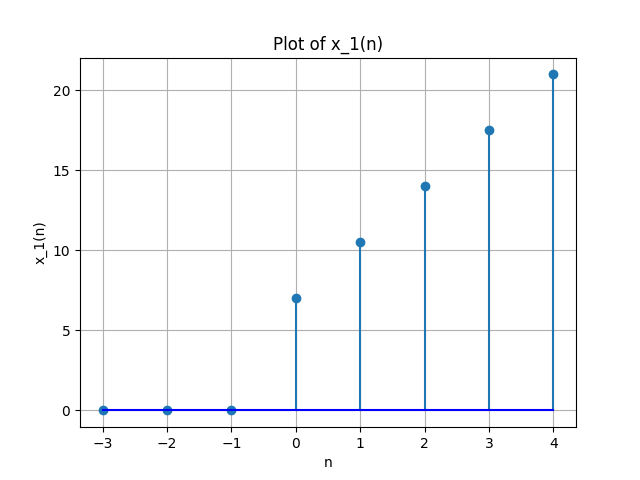
\includegraphics[width=12cm, height=8cm]{graph_1}
\caption{ $x_1(n)$ vs n }
\label{graph:ee25-g2}
\end{figure}
\vspace{0.5cm}


\begin{enumerate}
\vspace{0.5cm}
\item[(ii)]
 34 + 32 + 30 ... + 10
\vspace{0.5cm}

Using \ref{table:ee25-tab1} :
\begin{align}
x_2(n) &= (x_2(0) + nd_2)u_{(n)}\\
     10 &= 34 -2n\\
     n &= 12 
     \end{align}
\end{enumerate}

\begin{enumerate}
\item[1)] 
Calculating $s_2(12)$ :
For calculating the sum , we use the table \ref{table:ee25-tab1}
\begin{align}
 s_2{(12)} &= \frac{13}{2}(64+11(-2))\\
 s_2{(12)} &= 286.
 \end{align}
    \vspace{0.5cm}
\end{enumerate}

\begin{enumerate}
\item[2)] 
Z-Transform of $x_2(n)$ :
Using $\eqref{eq:ztrans}$
\begin{align}
X_2(z) &= \sum_{n=-\infty}^{\infty}(x_2(0) -2n)u_{(n)}Z^{-n} \\
 X_2(z) &= 34z(z-1)^{-1}-
       2z((z-1))^{-2} \label{eq:ee25-6}\\
\quad \abs {z}>\abs{1} 
\end{align}
\end{enumerate}


\begin{enumerate}
\item[3)]
Z-Transform of $s_2(n)$ :
Using table $\ref{table:ee25-tab1}$ and assuming 
\begin{align}
         h[n] &= u[n] \\
    y_2(n) &= x_2(n) * h(n) \\
    y_2(z) &= X_2(z) * H(z)
    \end{align}
    Where $X_2(z)$ comes from $\eqref{eq:ee25-6}$ and $H(z)$ from $\eqref{eq:ee25-9}$.
    For $y_2(z)$ :
    \begin{align}
            y_2(z) &= 34z(z-1)^{-1}-
       2z((z-1))^{-2})z(z-1)^{-1}
    \end{align}
    ROC:
    \begin{align} 
\quad \abs {z}>\abs{1} 
    \end{align}
\end{enumerate}

    \begin{enumerate}
    \item[4)]
Inversion of $y_2(z)$ :
By using partial fractions 
\begin{align}
    y_2(z) = \notag34(1-z^{-1})^{-1} + 34z^{-1}(1-z^{-1})^{-2} - (z^{-2} + z^{-1})(1-z^{-1})^{-3} - z^{-1}(1-z^{-1})^{-2}  
\end{align}
Using \eqref{eq:11.9.5.26.2} , \eqref{eq:11.9.5.26.3} and \eqref{eq:ee25-9} for inverse Z-transforms :
\begin{align}
 y_2(n) &= (34(n+1) - n(n+1))u(n)   
\end{align}
\end{enumerate}



\begin{figure}[!ht]
\centering
  \graphicspath{ {figs/} }
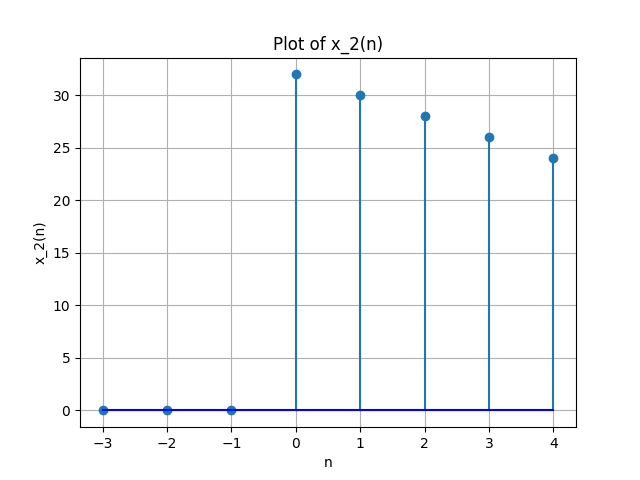
\includegraphics[width=12cm, height=8cm]{graph_2}
\caption{$x_2(n)$ vs n }
\label{graph:ee25-g3}
\end{figure}

\begin{enumerate}
\vspace{0.5cm} 
\item[(iii)]
-5 + -8 + -11 ... -230
\vspace{0.5cm}
\end{enumerate}

\begin{enumerate}
Using \ref{table:ee25-tab1}
\begin{align}
x_3(n) &= (x_3(0) -3n)u_{(n)}\\
-230 &= -5 -3n \\
n &= 75
\end{align}
\item[1)]
Calculating $s_3(75)$ :
Using \ref{table:ee25-tab1} :
\begin{align}
    s_3(75) &= \frac{76}{2}(-10+(76-1)(-3))\\
   s_3(75) &= -8930
    \end{align}
    \end{enumerate}

\begin{enumerate}
\item[2)] 
Z-Transform of $x_3(n)$ :
Using $\eqref{eq:ztrans}$
\begin{align}
X_3(z) &= \sum_{n=-\infty}^{\infty}(x_3(0) -3n)u_{(n)}Z^{-n} \\
X_3(z) &=  -5z(z-1)^{-1}-
       3z((z-1))^{-2} \label{eq:ee25-8}\\
\quad \abs {z}>\abs{1} 
\end{align}
\end{enumerate}

\begin{enumerate}
    \vspace{0.5cm}
\item[3)]
Z-Transform of $s_3(n)$ :
Using table $\ref{table:ee25-tab1}$ and assuming 
\begin{align}
         h(n) &= u(n) \\
    y_3(n) &= x_3(n) * h(n) \\
    y_3(z) &= X_3(z) * H(z)
    \end{align}
    Where $X_3(z)$ comes from $\eqref{eq:ee25-8}$ and $H_(z)$ from $\eqref{eq:ee25-9}$.
    For $y_3(z)$ :
    \begin{align}
            y_3(z) &= (-5z(z-1)^{-1}-
       3z((z-1))^{-2})z(z-1)^{-1}
    \end{align}
    ROC:
    \begin{align} 
\quad \abs {z}>\abs{1} 
    \end{align}
    \end{enumerate}

\begin{enumerate}
    \item[4)]
Inversion of $y_3(z)$ :
\begin{align}
    y_3(z) = \notag(-5(1-z^{-1})^{-1} - 5z^{-1}(1-z^{-1})^{-2} - (1.5)(z^{-2} + z^{-1})(1-z^{-1})^{-3} - (1.5)z^{-1}(1-z^{-1})^{-2}  
\end{align}
Using \eqref{eq:11.9.5.26.2} , \eqref{eq:11.9.5.26.3} and \eqref{eq:ee25-9} for inverse Z-transforms :
\begin{align}
 y_3(n) &= (-5(n+1) - 1.5n(n+1))u(n)   
\end{align}
\end{enumerate}


\begin{figure}[!ht]   
\centering
\graphicspath{ {figs/} }
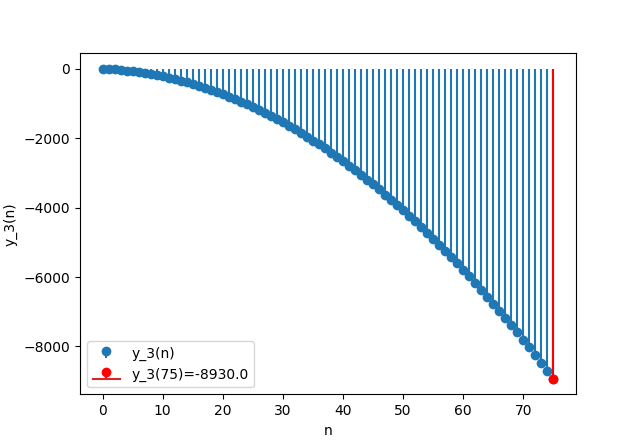
\includegraphics[width=12cm, height=8cm]{graph_3}
\caption{$x_3(n)$ vs n }
\label{graph:ee25-g4}
\end{figure}
 
\end{document}
